\documentclass{article}
\usepackage{hyperref, graphicx, floatrow}

\usepackage[letterpaper, margin=1in]{geometry}
\setlength{\parskip}{\baselineskip}
\setlength{\parindent}{0pt}


\title{Lhyra: Learned HYbrid Recursive Algorithms}

\author{
    Josh Gruenstein\\\texttt{jgru@mit.edu} \and Lior Hirschfeld\\\texttt{liorh@mit.edu} \and
    Benjamin Spector\\\texttt{spectorb@mit.edu}
}

\date{6.890 Spring 2019 Final Project}

\begin{document}

\maketitle

\section{Introduction}
A large number of computer science problems lend themselves naturally to recursive solutions. Of these, if more than one known algorithm exists, choosing between them may be difficult. Even if asymptotic, worst-case run time is known, this may have no bearing on real world use cases, which oftentimes operate on small inputs or data that is not representative of the entire space. Generally, a decision tree is chosen manually by an expert, who benchmarks the performance of each algorithm and selects whichever appears to perform most efficiently. A clear example of this is in the C++ STL, in which the standard algorithm is Introsort, which calls Quicksort until hitting a certain recursion depth, where it switches to Heapsort. This approach is far from ideal, not only because it is so time consuming, but also because decision making will be restricted only to those features which the expert tested most rigorously. 

Instead, we propose that this process should be automated through the introduction of machine learning. For this project, we designed and implemented Lhyra, a framework designed to automatically find efficient recursive trees given arbitrary solvers, data distributions, and optimization criteria. Lhyra was largely inspired by Professor Kraska's work on learned B-Trees and the Recursive Model Index \cite{kraska}, as we believed that, through high-level abstractions, it might be possible to apply a similar methodology to a large number of recursive data structures and algorithms. Below, we discuss Lhyra's components in more detail and present our results when applying Lhyra to two common problems, \textsc{Closest Pair} and \textsc{Sorting}.


\section{Framework}
A Lhyra instance is described by the following components:

\begin{itemize}
	\item \textbf{Bag of Solvers $S$.} Each solver $s_i \in S$ is equipped to solve an instance of the problem at hand, potentially by calling the Lhyra instance on sub-problems. Each solver $s_i$ may also have a set of hyper-parameters $h_{ij}$. 

	\item \textbf{Data Generator / Training Data Set $D$.} In the training phase the problems in this set / generated by this generator are used by the optimizer to learn how to select a solver $s_i$ from S given problem features.

	\item \textbf{Feature Extractor $F(x)$.} Our goal is to learn how to select the ideal solver based on a given input, thus we need a nice way of extracting useful features about an input. For example, a feature extractor for a sorting Lhyra instance may return a vector containing the length of the list, number of unique elements, and how sorted it already is. Defaults to a vector of length 1 containing the depth of the recursion.

	\item \textbf{Optimizer $O$.} Given a feature extractor, a training data set, and a bag of solvers, the optimizer learns how to select a solver given a vector of problem features.  Optimizers should default to minimizing computation time and/or memory, but can take an arbitrary cost function $C(x,y)$ that produces some cost to be minimized given a problem and solution. 
\end{itemize}

Once initialized, a call to a Lhyra instance solves a problem $x$ through the following steps:

\begin{enumerate}
	\item Compute $F(x)$.
	\item Pass $F(x)$ into the solver selector learned by the optimizer, which returns a parametrized solver $s_{ih}$.
	\item Compute $s_{ih}(x)$.
	\begin{enumerate}
		\item For each sub-problem $y_i$ identified by $s_{ih}$, repeat the above process.
		\item Combine the sub-problems and return a result.
	\end{enumerate}
\end{enumerate}

An ideal solver selector and feature extractor would be fast enough for the benefits gained by ideal solver selection to outweigh the additional overhead. After implementing Lhyra in both Python and C++, we found relative performance to be very impacted by language choice and implementation specifics.

\subsection{Optimizers}

The optimizer carries the responsibility of selecting the ideal solver, and training the model to perform said selection process.  An ideal Lhyra optimizer would satisfy the following conditions:

\begin{itemize}
    \item \textbf{Applicability.} The optimizer must learn using data that accessible. For example, gradient descent may be impossible if the relationship between input and cost is unclear.
    \item \textbf{Flexibility} Given a feature vector, the optimizer must be able to apply a sufficiently complex matching to extract meaningful data for solver selection.
    \item \textbf{Speed.} The optimizer must predict quickly enough that its overhead does not outweigh gains from selecting the proper solver. This component can be ignored if time is not an optimization criteria.
\end{itemize}

Although each optimizer we experimented with used a different training process, we decided to use a common overall framework in generating feedback times (our optimizer cost function $C$).  We chose to measure the entire time to execute a sub-problem, including recursive calls to (potentially different) solvers selected by Lhyra.  At face value, this is an odd choice compared to the far more straightforward method of simply measuring a solver's own execution time, not including that of its children.  It introduces strange cyclical dependencies, where Lhyra's choice of solver must depend on an ingrained understanding of its own decision making.  This also forces Lhyra's ``training'' process to be online, as timing measurements are only useful using the most up-to-date model parameters.

However, this is exactly the property we would want in an ideal optimizer.  Consider a solver which did minimal work, instead deciding to punt nearly all of the computation to its children.  A naive optimizer would unduly favor such a solver, and fail to recognize useful sequential relationships in solvers: for example, that solver B might be best following solver A.  Although this methodology is harder to train, it is ideal presuming the model is able to converge at all (which we empirically do with some optimizers). 

\subsubsection{Neural Network Classifiers}

A natural optimizer architecture might feed our feature vector through a neural network, which outputs a one-hot vector representing solver selection. As we can make this neural network arbitrary large, this system is guaranteed to satisfy our condition of flexibility. However, it suffers in other respects.  As our classifier gets larger, classification latency would suffer.  Techniques designed to speed up neural network execution (such as GPUs) largely rely on batching for speed and are do not significantly improve latency for single inferences, limiting the size of potential networks.

Training is also a challenge. Gradient descent is incompatible with this architecture, because there exists no discernible relationship between network weights and cost: without exhausting all available options, it is impossible to determine whether the ideal solver was selected.  We attempted to train a single perceptron classifier using REINFORCE \cite{reinforce}, a member of the policy gradients family that uses reward signals to estimate a classifier gradient.  However, we found our classifier was unable to converge on reasonable solutions, as the estimated gradients were far too noisy.

We were able to obtain somewhat reasonable results training the same model from above using naive hill-climbing, randomly perturbing weights and keeping perturbations that led to performance improvements.  However, our results were outperformed by better optimizers (such as our linear regressor), and we do not think this training method would scale to different and more complex problems due to its fragility.

\subsubsection{Linear Regressors}

An alternative architecture trains a set of linear regressors, where each predicts execution costs for a call-tree starting at a certain solver type.  For any given feature vector, the optimizer predicts with each regressor and selects the solver corresponding to the regressor with smallest output. Each regressor can be easily trained through linear least-squares.

The primary concern with this method is that it lacks flexibility. With only a single perceptron, a linear regressor lacks the ability to extract nonlinear relationships between features. For both \textsc{Closest Pair} and \textsc{Sorting}, we did not find this was not problematic, but this deficiency should be considered when solver selection is more complex. One could imagine remedying this issue either with automatic feature extraction or a more powerful (non-linear and non-convex) regressor.

Even with a convergent optimizer, we struggled with overhead from running our regressors.  For example, in order to make the overhead on recursive calls in our Python implementation net-positive, we had to perform micro-optimizations such as swapping out Scikit-learn's \texttt{LinearRegression} \cite{sklearn} class's inference methods for our own. 

\section{Experiments}

In order to develop and test Lhyra, we built implementations in both Python and C++.  We will  show here results from C++ benchmarks, as we found relative performance measurement to be difficult in Python due to overhead such as garbage collection.

\subsection{Closest Pair of Points}

Consider the \textsc{Closest Pair} problem, in which given a set of $n$ points $P$ you must identify a pair of unique points $(p_i,p_j)$ to minimize distance $||p_i - p_j||_2$.  This is a common problem, but not quite common enough for hyper-optimized hand-coded adaptive implementations to exist.  However, there are two common algorithms for solving this problem.

\begin{enumerate}
    \item \textbf{Brute force.}  In $O(n^2)$ time, exhaustively enumerate all possible pairs of points, and choose the one with the smallest distance.
    \item \textbf{Divide \& conquer.}  Partition the points by the median $x$ coordinate, and recurse on the points to the left and right of the dividing line, $P_l$ and $P_r$ respectively.  Then, for each point within $\min(d(P_r),d(P_r))$ of the dividing line, enumerate all possible pairs to see if one has a shorter distance than $d(P_r)$ or $d(P_l)$, where $d$ is the smallest pair distance in that set.  It can be shown geometrically that the number of pairs within this distance of the dividing line is $O(n)$ \cite{clrs}, so the algorithm overall is $O(n\log n)$.
\end{enumerate}

We implemented a Lhyra instance with the above two solvers, using our linear regressor-based optimizer and extracting set size $n$ as our only feature.  With only seconds of training, Lhyra was able to substantially outperform both algorithms for nearly all $n$ by learning to use the divide-and-conquer method at high $n$, and the brute-force method at lower $n$.

\vspace{0.5cm}
\begin{figure}[!h]
    \centering
    \begin{floatrow}
        \ffigbox{
            \caption{\textsc{Closest Pair} training curve}
        }{
            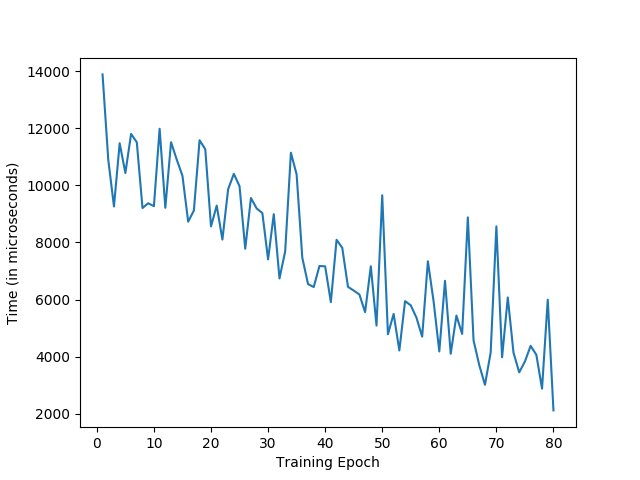
\includegraphics[width=8cm]{images/training_times_points}
        }
      
        \ffigbox{
            \caption{\textsc{Closest Pair} relative performance}
        }{%
            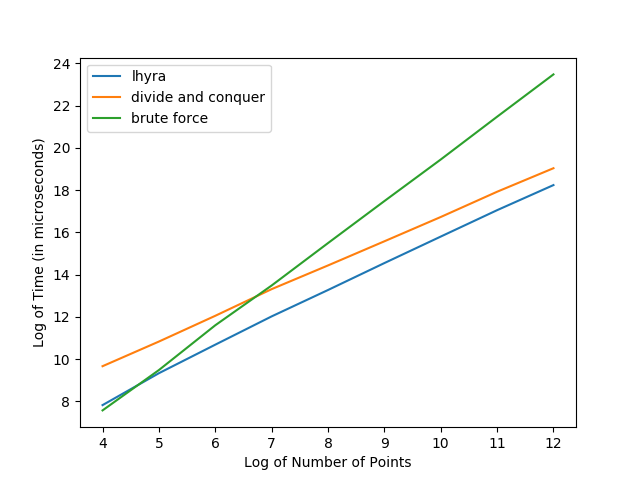
\includegraphics[width=8cm]{images/relative_plot_points}
        }
    \end{floatrow}
\end{figure}

\subsection{List Sorting}

A more complex recursive problem is \textsc{Sorting}, producing an ordered list from a potentially unordered one.  We chose the following common sorting methods for our bag of solvers: Insertion Sort ($O(n^2)$), Merge Sort ($O(n \log n)$), and Quicksort (also $O(n \log n)$). Due to their ubiquity, we will not review how these algorithms work.

We implemented a Lhyra instance with the three solvers, the same optimizer as above, and two features: the list length $n$, and sortedness $n*s$, calculated in $O(1)$ time by randomly sampling 10 elements from the list and checking their orderedness $s$, then multiplying by $n$ to normalize to our other feature.  Below are results from this instance using purely-random lists, showing that Lhyra dramatically outperforms the fastest algorithm Quicksort at large $n$, and matches Insertion Sort at small $n$.

\vspace{0.5cm}
\begin{figure}[!ht]
    \centering
    \begin{floatrow}
        \ffigbox{
            \caption{Random \textsc{Sorting} training curve}
        }{
            \includegraphics[width=5.5cm]{example-image}
        }
      
        \ffigbox{
            \caption{Random \textsc{Sorting} relative performance}
        }{%
            \includegraphics[width=5.5cm]{example-image}
        }
    \end{floatrow}
\end{figure}

However, Lhyra can perform even better with interesting and changing data distributions.  Take the following example, where lists are already 50\% sorted.

\vspace{0.5cm}
\begin{figure}[!ht]
    \centering
    \begin{floatrow}
        \ffigbox{
            \caption{Partially-sorted \textsc{Sorting} training curve}
        }{
            \includegraphics[width=5.5cm]{example-image}
        }
      
        \ffigbox{
            \caption{Partially-sorted \textsc{Sorting} relative performance}
        }{%
            \includegraphics[width=5.5cm]{example-image}
        }
    \end{floatrow}
\end{figure}

Lhyra learns that our implementation of Insertion Sort is $O(n)$ on sorted lists, and dynamically exploits that knowledge to widen its performance gap against other solvers.

\section{Discussion}

% parametrizing solvers: random variables, etc
% learned feature extraction
One potential future optimization is pruning the \textit{Optimizer}. Shrinking the network's size would save time with each prediction, perhaps resulting in a significant speedup over many recursive calls. This process would also inform us of useless features. If any edges attached to the input are deleted from the network during pruning, then we can automatically remove the corresponding feature from the \textit{Feature Extractor}, resulting in additional performance gains.

A natural extension of Lhyra is introducing learned feature extraction. This process may involve combining the \textit{Feature Extractor} and \textit{Optimizer} components. Instead of passing in a feature vector to the \textit{Optimizer}, it receives raw data as input. For example, if operating on a graph, we could make use of Message Passage Neural Networks, which have recently been shown to dramatically improve performance over traditional features on tasks like molecular property prediction \cite{GilmerSRVD17}. Clearly, this process would require more computation, so this method would likely only be worthwhile on tasks where cost is lessened dramatically by good solver selection.

An application of Lhyra which we have not yet explored is online learning in production environments.  If the data distribution changes over time, Lhyra could continuously use evaluation data to train its solver picker.  This is actually doable for both \textsc{Sorting} and \textsc{Closest Pair}, as training for the whole dataset occurs in seconds, so miniature iterative updates could easily be done in production while remaining net-positive.

We would also like to investigate Lhyra's effectiveness at optimizing criteria other than time. One option would be to explore polynomial time approximation algorithms to NP-hard problems. In this scenario, cost could be a weighted function of evaluation time and accuracy, depending on the priorities of the user.

\bibliographystyle{unsrt}
\bibliography{ref}

\appendix
\section{Code and Reproducibility}

Our research codebase is available under the MIT license at the below Github repository.  Our code structure is described in the file \texttt{README.md}.

\begin{center}
\url{https://github.com/joshuagruenstein/lhyra}
\end{center}

In order to maximize reproducibility, we bundled our codebase into a Docker container, and set up Continuous Integration through Travis CI to auto-generate plots whenever we push to our Github repository.  Thus, we have a transparent, reproducible pipeline for obtaining results with Lhyra.  You can check out the figures generated by our most recent commit by going to the following link, and navigating to the \texttt{i.imgur.com} links at the bottom of the console output.

\begin{center}
\url{https://travis-ci.org/joshuagruenstein/lhyra}
\end{center}



\end{document}